\chapter{Results and conclusion}

In this chapter, the signal, background and data yields after applying full selections are used to determine the upper limits of the production cross section of $Z'$. The 95\% confidence-level limit on the signal contribution in the data is computed by the $CL_{s}$ method\cite{CLs1,CLs2} with the RooStats\cite{RooStats} package. In order to extract the limit on the production cross section times the branching ratios, the CMS standard combination tool\cite{HiggsCombineTool} has been used. Moreover, the Asymptotic method is used to calculate preliminary 95\% C.L. upper limits with 1$\sigma$ and 2$\sigma$ bands using the $CL_{s}$ frequentist calculation currently recommended by the LHC Higgs Combination Group.

\section{Exclusion limit results}

\subsection{Counting result}
The expected exclusion limits with the $\pm$1 and $\pm$2 $\sigma$ band, obtained by the provided event yield information, are reported in Fig.~\ref{fig:LimitResult} (a) in terms of upper limits on the signal cross section.

\subsection{1D shape result}
In addition to the event yield information, the $m_{Zh}$ distributions of predicted signal, background and data are provided. All the statistical and systematics uncertainties (with shape uncertainties) are included. The result is shown in Fig.~\ref{fig:LimitResult} (b).

\subsection{2D shape result}
Both the CSV shape and the $m_{Zh}$ spectrum are considered in this strategy. Therefore the systematics related to the CSV shape are also introduced. The result is shown in Fig.~\ref{fig:LimitResult} (c).

\section{Conclusion}
Since no excess above the expected SM background was found, the result is interpreted as an exclusion limit on the production cross section times the branching ratio in the Zh channel as a function of the resonance mass.

Inspecting the limit result, the counting method shows no sensitivity on the cross section limit plot. The expected (observed) lower bound on the $Z'$ mass obtained in the 1D limit result (top figure) is 1257 (1350) GeV, while the 2D result gives 1528 (1477) GeV. The 2D method has improved the limits significantly.

Finally, this analysis puts an upper limit at 95\% confidence level on the cross section of $pp\rightarrow Z'\rightarrow Zh$ at $\sqrt{s}$ = 8 TeV. The maximal expected (observed) limit result of 1528 (1477) GeV is determined.

\begin{figure}[hbtp]
  \subfigure[Counting result]{
    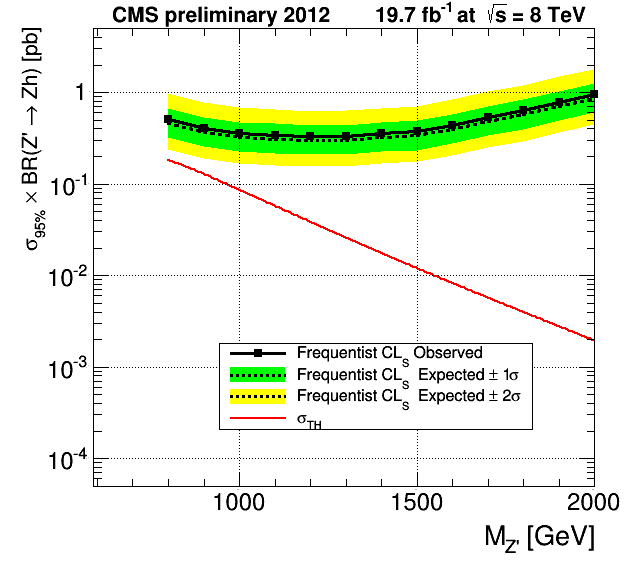
\includegraphics[width=0.5\textwidth]{figure/CH4/XZH_counting_Asymptotic_log.png}}
  \subfigure[1D shape result]{
    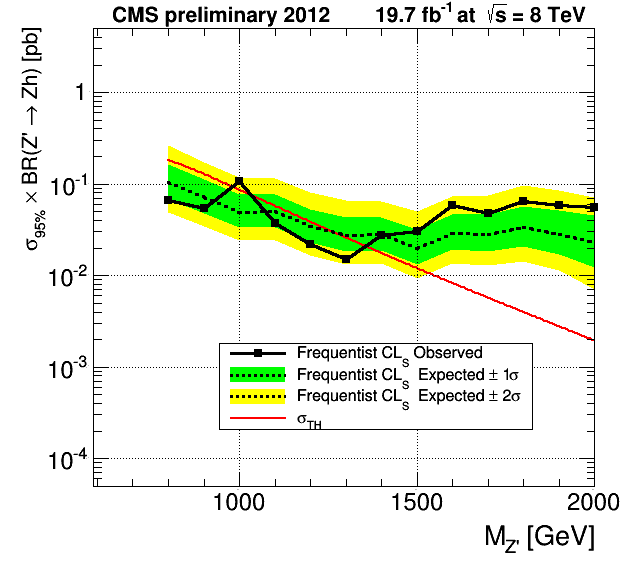
\includegraphics[width=0.5\textwidth]{figure/CH4/XZH_shape1d_Asymptotic_log.png}}
  \begin{center}
  \subfigure[2D shape result]{
    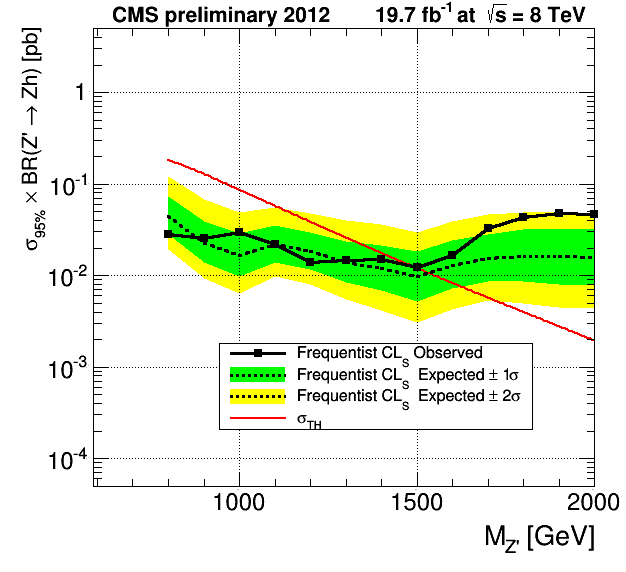
\includegraphics[width=0.5\textwidth]{figure/CH4/XZH_shape2d_Asymptotic_log.png}}
  \end{center}
  \caption{\label{fig:LimitResult} Observed and expected (with $\pm$1(2)$\sigma$ band) 95\% C.L. upper limit on $\sigma \times$BR($Z'\rightarrow Zh$) including all statistical and systematics uncertainties.}
\end{figure}


